\chapter{CertOS Runtime Assurance}
\label{ch:certos-runtime-assurance}

\section{CertOS as release semantics}
CertOS is the part of ORIUS that turns repaired action into a governed runtime object.
Without lifecycle state, fallback rules, and an audit chain, certificates would be inert
metadata. With CertOS, certificate validity becomes part of the release decision itself:
which action was allowed, under which reliability state, for which horizon, with which
fallback if the certificate expires or becomes invalid?

This is the point at which the ORIUS kernel acquires operational semantics.
\texttt{DomainAdapter} defines the local safety predicate and fallback object that CertOS
must protect, and the universal benchmark schema defines the replay traces from which
certificate validity, latency, and lifecycle behavior are evaluated. In that sense, CertOS
is the computational bridge between repaired action and a safety argument that can later be
audited.

\section{Lifecycle invariants}
The lifecycle logic is narrow and strong. A protected action is never released without a
valid certificate or an explicit fallback. Certificate state must be renewable, expirable,
revocable, and auditable. Runtime traces must preserve enough information to reconstruct why
the release was allowed and when the governing assumptions ceased to hold. These are not
administrative conveniences. They are the invariants that keep repaired action tied to a
reviewable safety argument.

\begin{figure}[htbp]
\centering
\IfFileExists{reports/publication/fig_orius_runtime_governance_matrix.png}{%
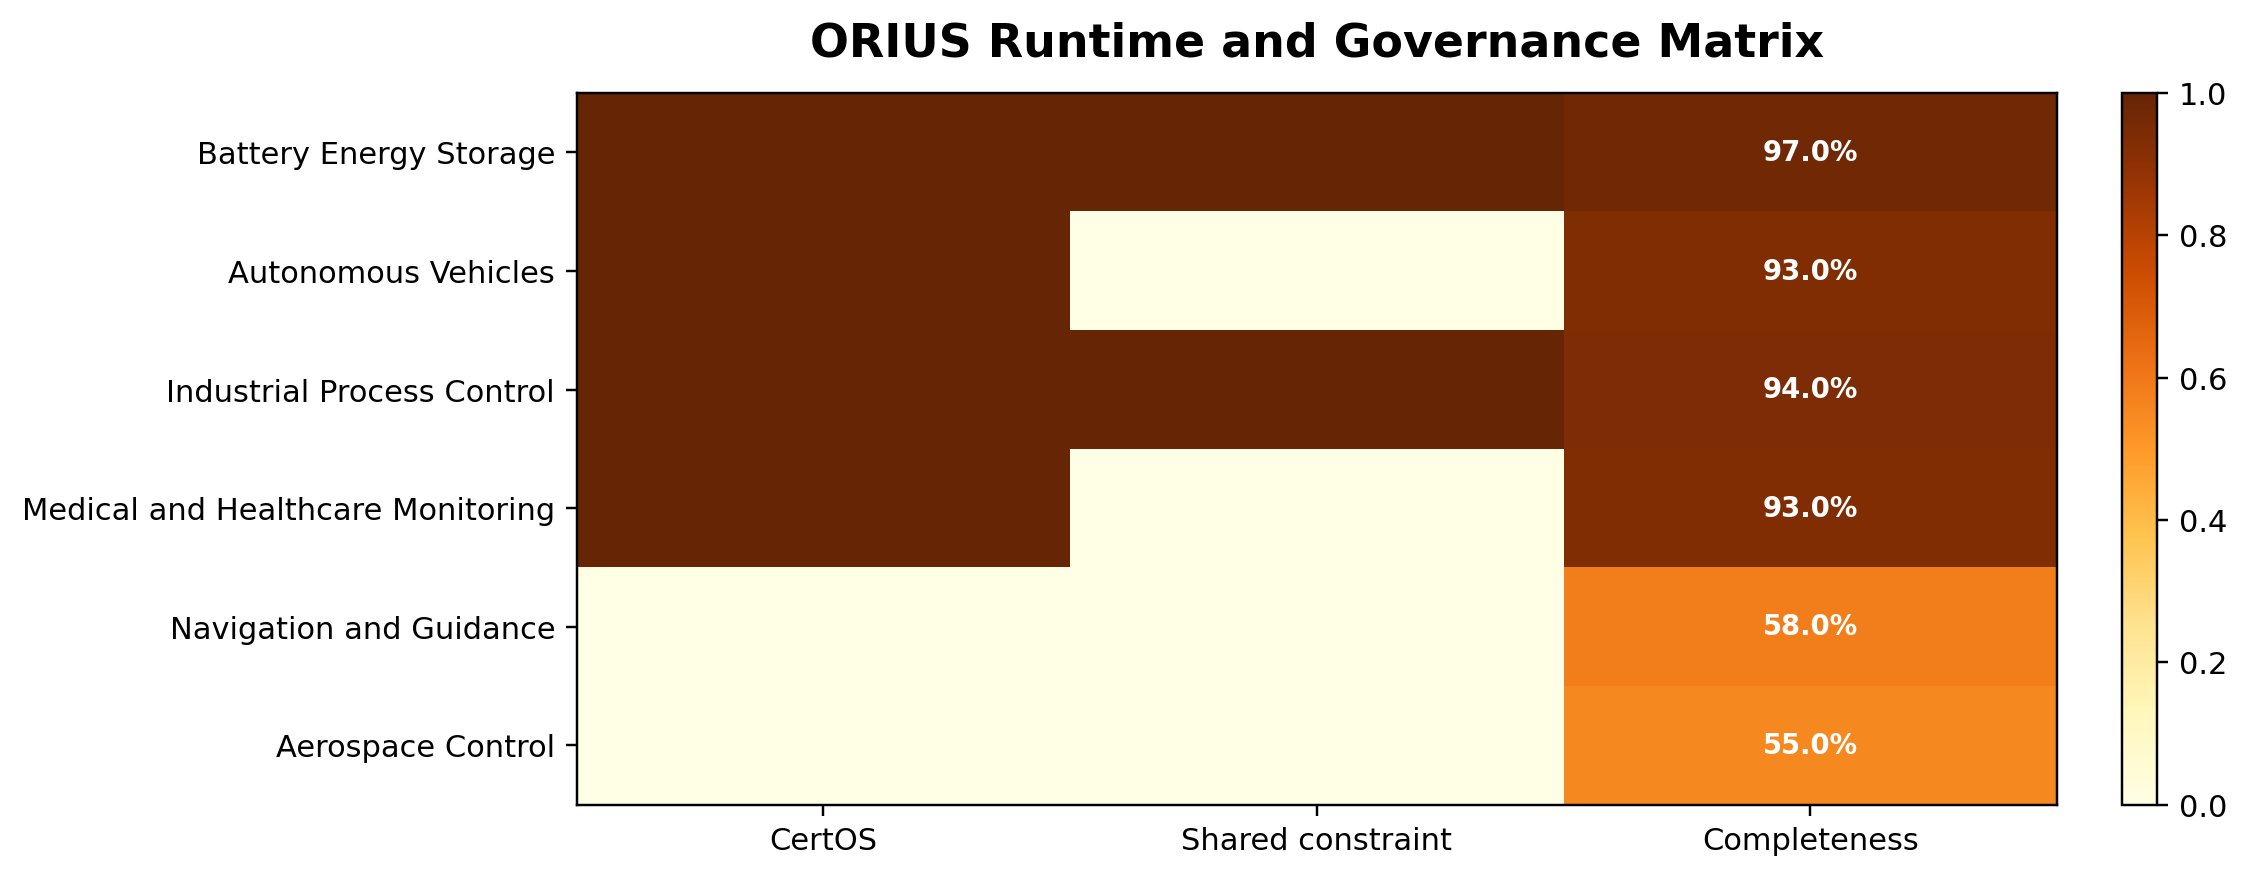
\includegraphics[width=0.88\textwidth]{reports/publication/fig_orius_runtime_governance_matrix.png}%
}{%
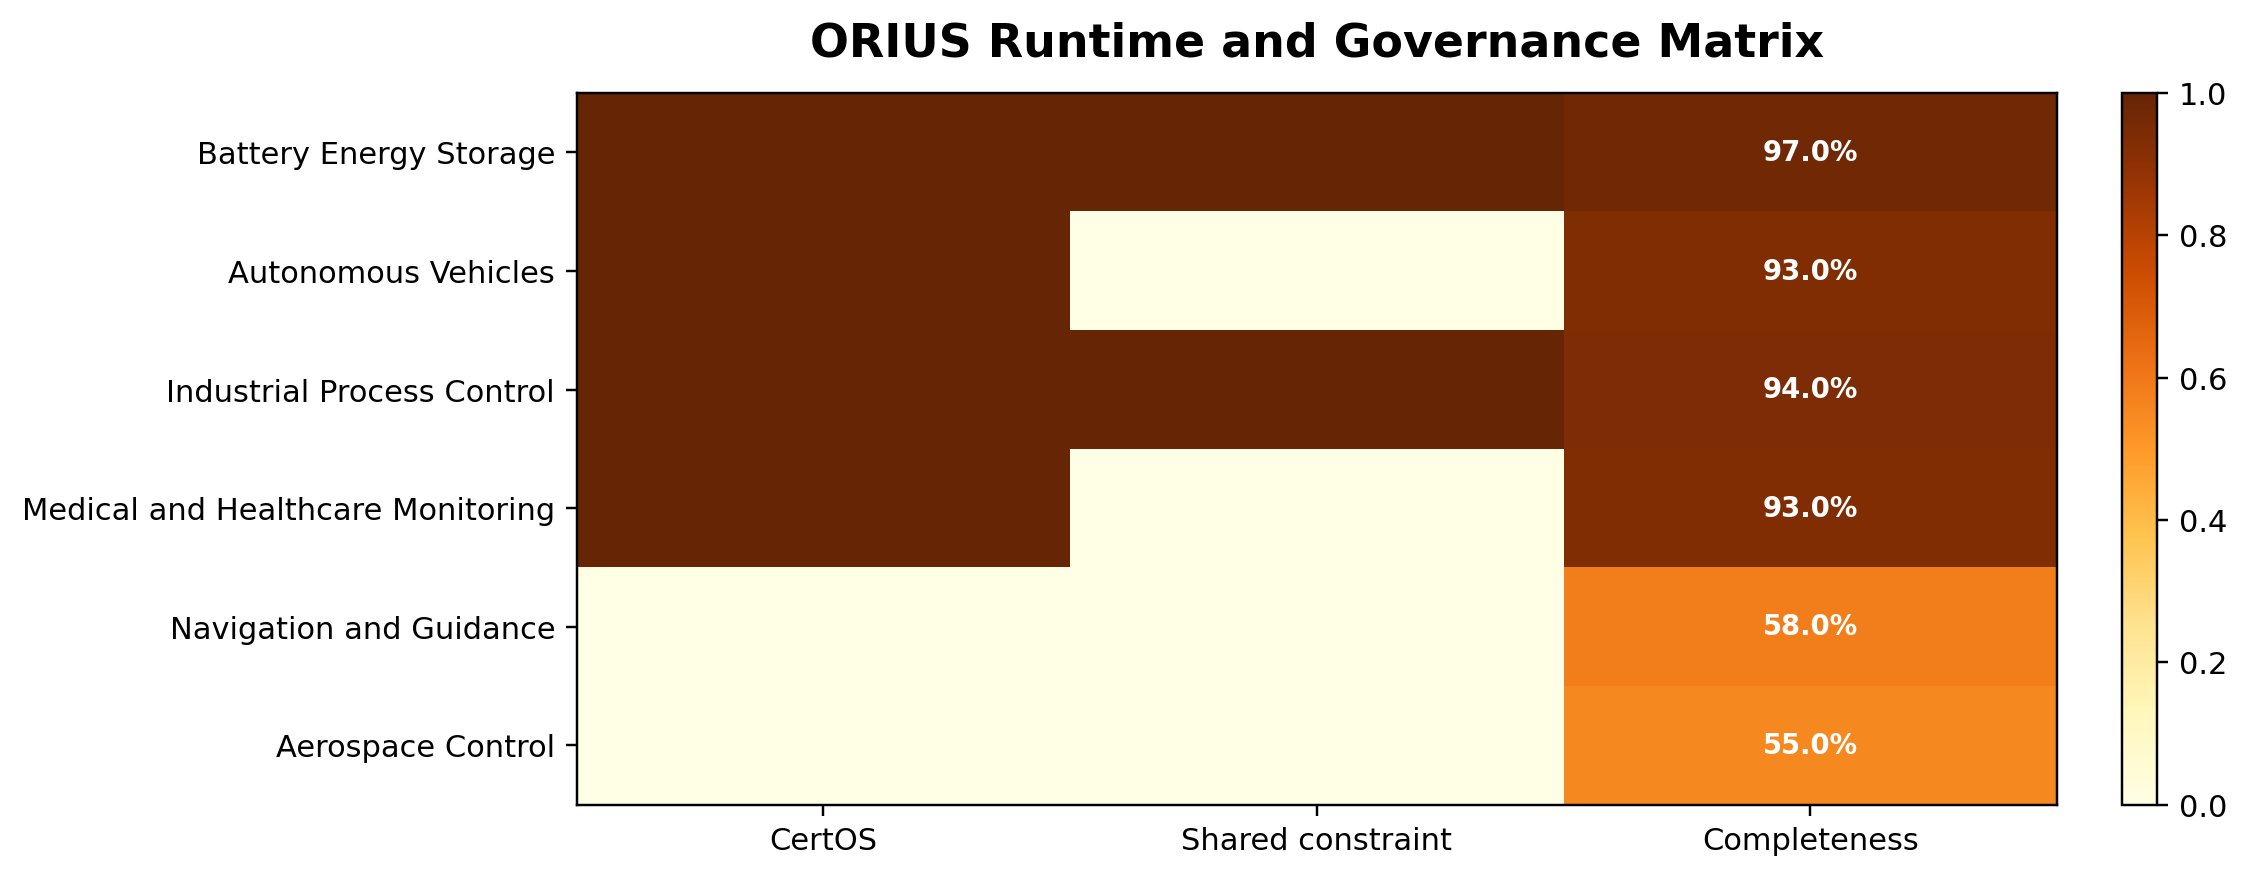
\includegraphics[width=0.88\textwidth]{../reports/publication/fig_orius_runtime_governance_matrix.png}%
}
\caption{CertOS lifecycle and runtime-governance surface across ORIUS domains. The figure
shows how certificate issue, validation, expiry, fallback, and audit continuity are exposed
as part of runtime safety rather than as post hoc reporting.}
\label{fig:runtime-governance-matrix}
\end{figure}

The figure highlights the right scientific point: governance is not separate from runtime
safety once release depends on repaired action under degraded observation. What varies across
rows is the maturity of the evaluated lifecycle surface, not the meaning of the lifecycle
itself.

\section{Architecture-level universality, evidence-tiered maturity}
CertOS is universal at the level of release semantics. Every defended ORIUS row needs a
certificate object, fallback policy, and audit trace. What is not yet universal is equal
deployment maturity across every domain. Battery, industrial process control, and healthcare
provide the strongest defended lifecycle surfaces. The autonomous-vehicle row shows a
defended bounded runtime surface under current artifacts. Navigation and aerospace remain
gated for the same empirical reasons already stated elsewhere in the dissertation. CertOS
therefore supplies one common governance object without pretending that all deployment
surfaces are equally mature today.

\section{Exact governance claim}
The CertOS claim is exact and intentionally narrower than a flat deployment slogan: ORIUS
provides a policy-driven runtime governance layer in which repaired action, fallback, and
certificate validity are coupled, auditable, and recoverable after the fact. That claim is
scientifically important because a runtime safety layer without release semantics cannot say
what action was justified once degraded observation has already entered the control loop.
